% Created 2020-06-30 Tue 06:27
% Intended LaTeX compiler: pdflatex
\documentclass[11pt]{article}
\usepackage[utf8]{inputenc}
\usepackage[T1]{fontenc}
\usepackage{graphicx}
\usepackage{grffile}
\usepackage{longtable}
\usepackage{wrapfig}
\usepackage{rotating}
\usepackage[normalem]{ulem}
\usepackage{amsmath}
\usepackage{textcomp}
\usepackage{amssymb}
\usepackage{capt-of}
\usepackage{hyperref}
\usepackage{color}
\usepackage{listings}
\usepackage[table,xcdraw]{xcolor}
\usepackage{listings}

% src: http://texdoc.net/texmf-dist/doc/latex/listings/listings.pdf
\lstdefinestyle{customc}{
  belowcaptionskip=1\baselineskip,
  breaklines=true,
  %frame=L,%lines, whole
  xleftmargin=\parindent,
  language=C,
  showstringspaces=false,
  basicstyle=\scriptsize\ttfamily,
  keywordstyle=\bfseries\color{green!40!black},
  commentstyle=\itshape\color{purple!40!black},
  identifierstyle=\color{blue},
  stringstyle=\color{orange},
  numberstyle={\tiny},
  numbers=left,
  numberblanklines=false,
  stepnumber=5,
  backgroundcolor=\color{yellow!10}, 
  frame=tlb
}

\lstdefinestyle{customasm}{
  belowcaptionskip=1\baselineskip,
  frame=L,
  xleftmargin=\parindent,
  language=[x86masm]Assembler,
  basicstyle=\footnotesize\ttfamily,
  commentstyle=\itshape\color{purple!40!black},
}

\lstset{escapechar=@,style=customc}

\author{José Miguel Alves Pires\thanks{a50178@alunos.uminho.pt}}
\date{\textit{<2020-06-30 Tue>}}
\title{cheatsheet}
\hypersetup{
 pdfauthor={José Miguel Alves Pires},
 pdftitle={cheatsheet},
 pdfkeywords={},
 pdfsubject={},
 pdfcreator={Emacs 26.3 (Org mode 9.3.6)}, 
 pdflang={English}}
\begin{document}

\maketitle
\tableofcontents


\section{Modular design}
\label{sec:org8053dba}
Modular design is useful to separate logical units inside the \LaTeX{} environment.
\begin{itemize}
\item \texttt{dissertation.tex}: main document that defines all the formatting and includes
all the relevant \texttt{.tex} documents
\item \texttt{./sty}: contains the stylesheets for the document, such as:
\begin{itemize}
\item \texttt{dissertation-xelatex.sty}: stylesheet for the main document
\item \texttt{listing.sty}: stylesheet for the listings to be formatted and presented
\end{itemize}
\item \texttt{./sec}: contains secondary files, like images, PDFs, acronyms and symbols
\item \texttt{./bib}: contains the bibliography database
\item \texttt{./listing}: contains the listings (code) to be displayed
\item \texttt{./font}: contains the fonts to be used
\item \texttt{./tex}: contains the \texttt{.tex} documents to be inputted, subdivided in:
\begin{itemize}
\item \texttt{Pre\_Chap}: Pre chapters (not used here)
\item \texttt{Chap}: chapters
\item \texttt{Append}: appendices
\end{itemize}
\end{itemize}

Regarding \texttt{.tex} documents, they can be included as follows (the extension
\texttt{.tex} is implicit):
\begin{itemize}
\item \texttt{\textbackslash{}input\{path/to/file\}}: inputs the file as is (\textsubscript{recommended}\_)
\item \texttt{\textbackslash{}include\{path/to/file\}}: inputs the file and adds an extra blank page at the
end.
\end{itemize}

\section{Sectioning}
\label{sec:org3020630}
Sectioning is used to define the logical structure of the document. The most
relevant commands are:
\begin{enumerate}
\item \texttt{\textbackslash{}chapter}: chapter
\item \texttt{\textbackslash{}section}: section
\item \texttt{\textbackslash{}subsection}: subsection
\item \texttt{\textbackslash{}subsubsection}: subsubsection
\item \texttt{\textbackslash{}paragraph}: paragraph
\item \texttt{\textbackslash{}subparagraph}: subparagraph
\end{enumerate}

\section{Floats}
\label{sec:org97c1215}
\subsection{Figures}
\label{sec:org515f4f5}
\lstset{language=[LaTeX]TeX,label= ,caption= ,captionpos=b,numbers=none}
\begin{lstlisting}
\begin{figure}[!ht]
\centering
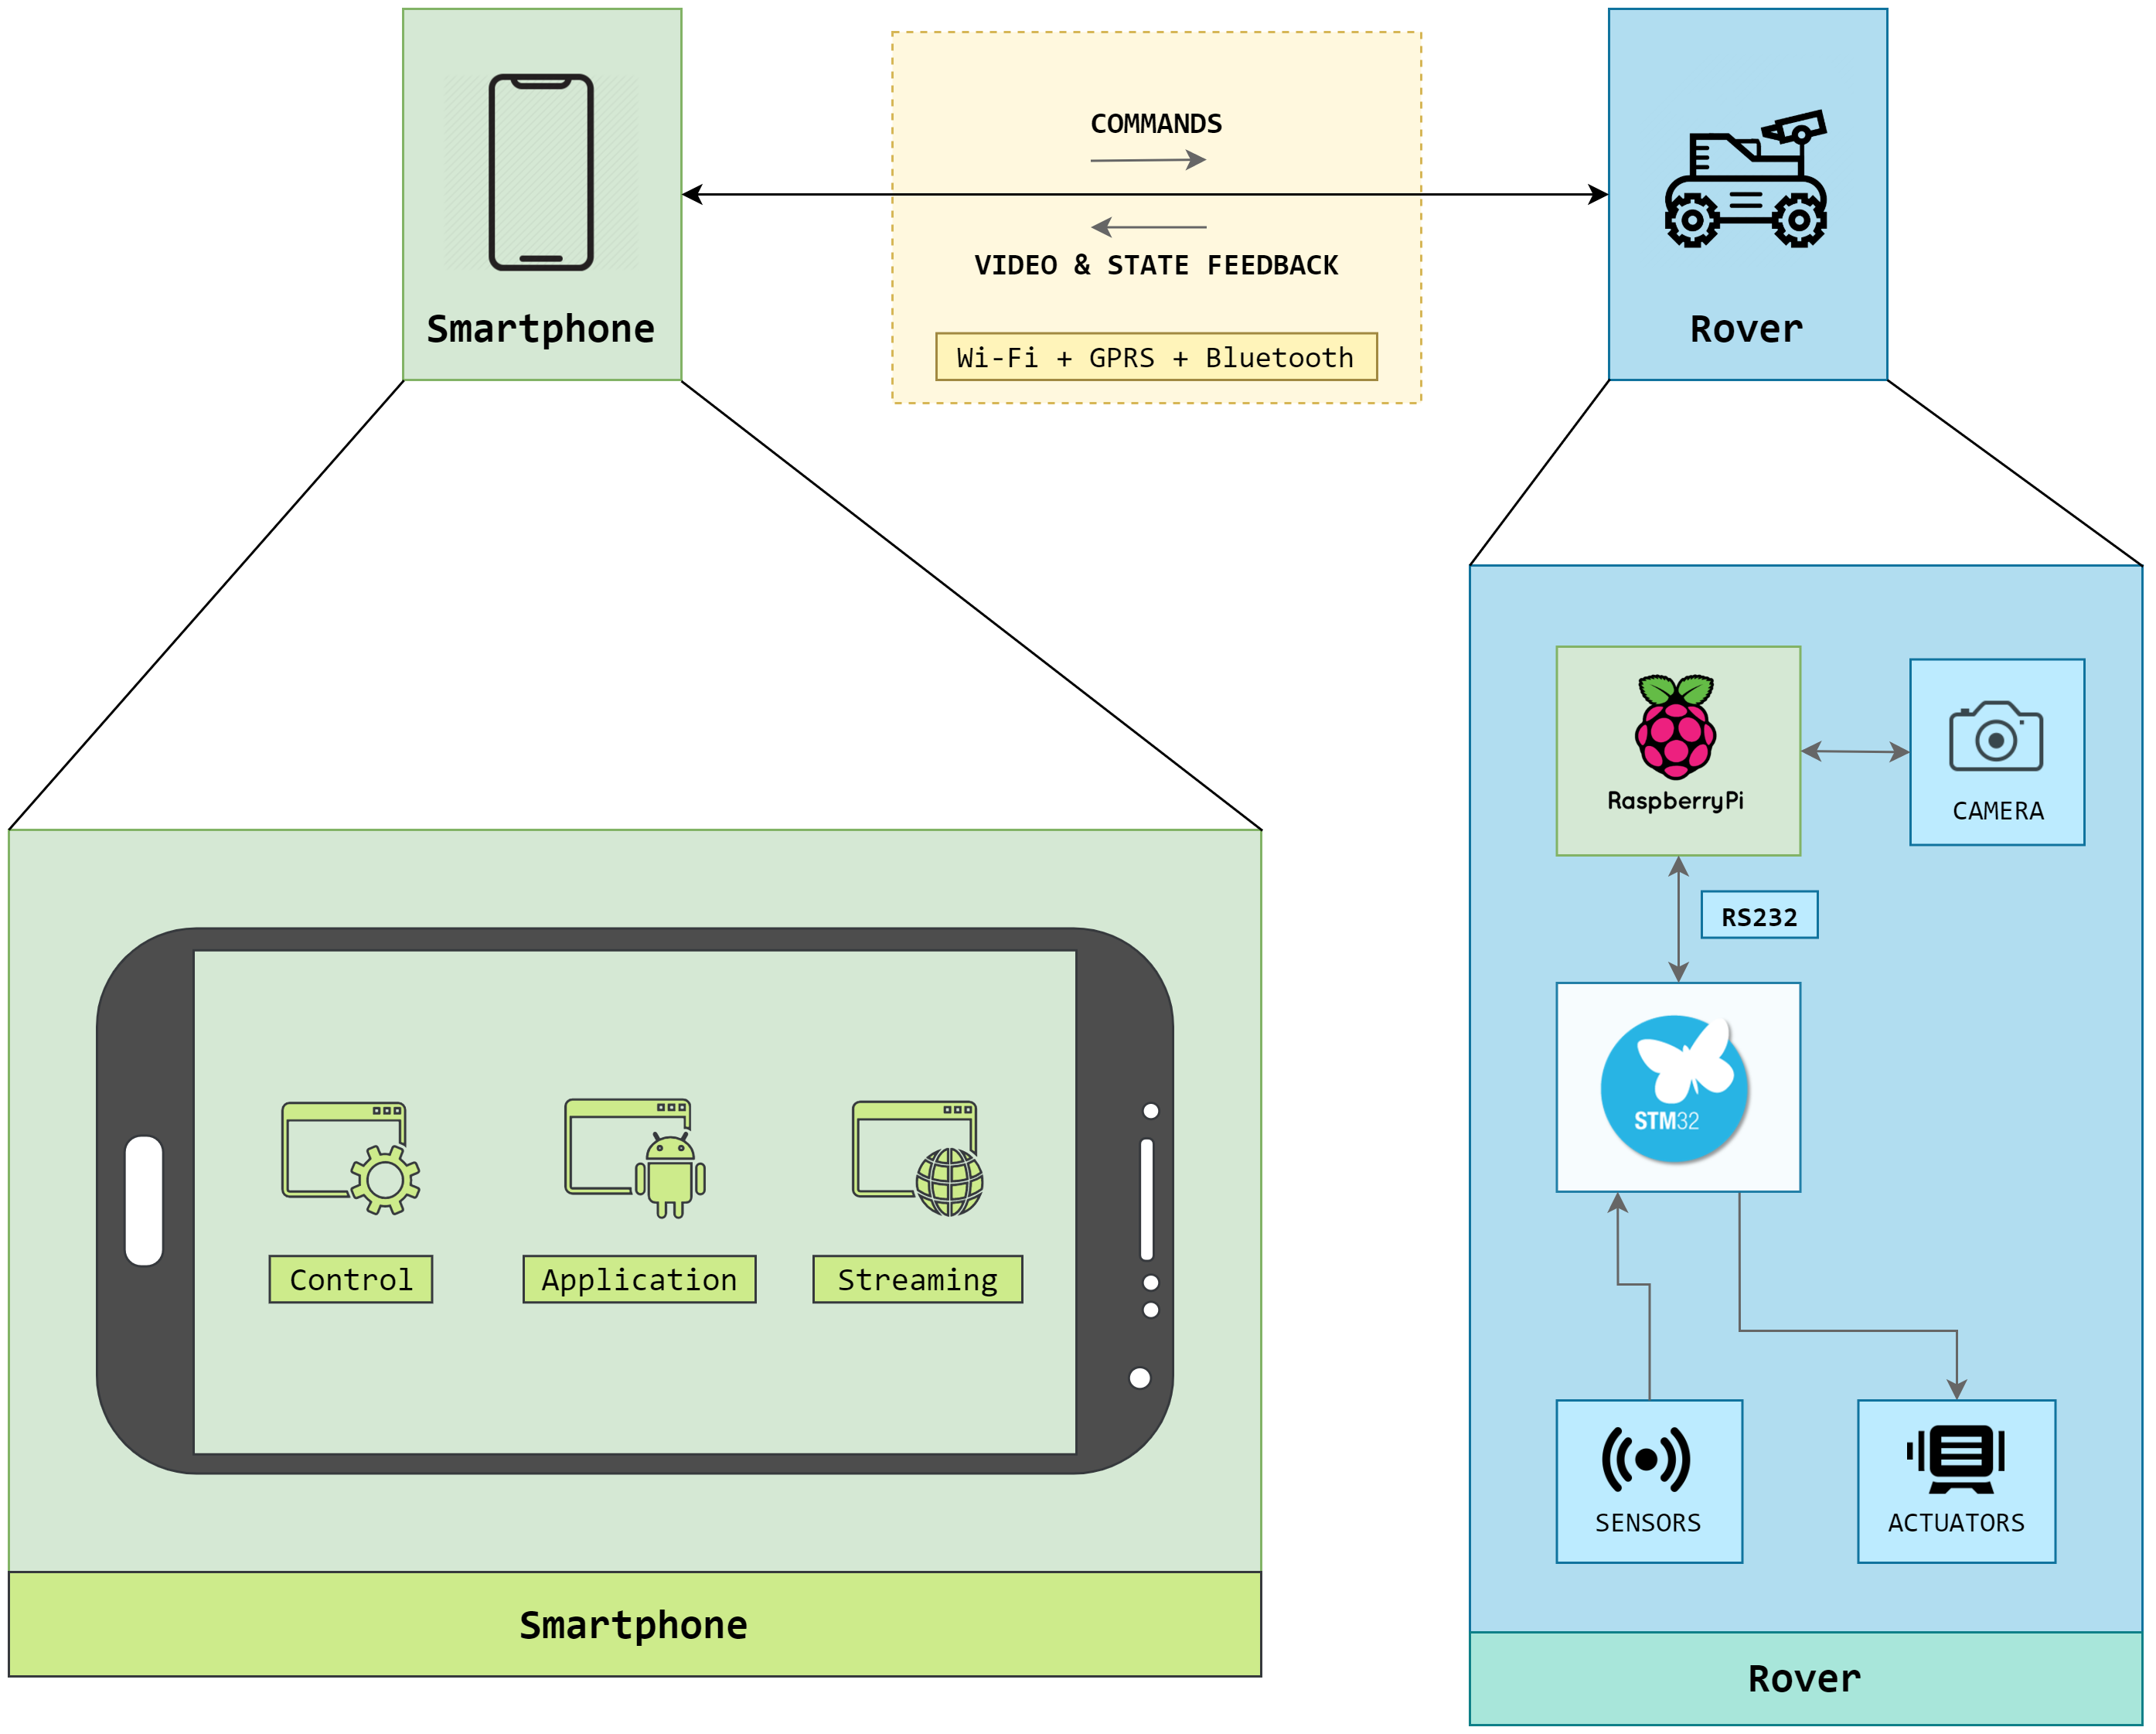
\includegraphics[width=1.0\textwidth]{./img/initial_design_diagram.png}
\caption{\label{fig:initial-design}Initial design: Block diagram view}
\end{figure}
\end{lstlisting}
\textbf{Result} (see Fig. \ref{fig:initial-design}):
\begin{figure}[!ht]
\centering
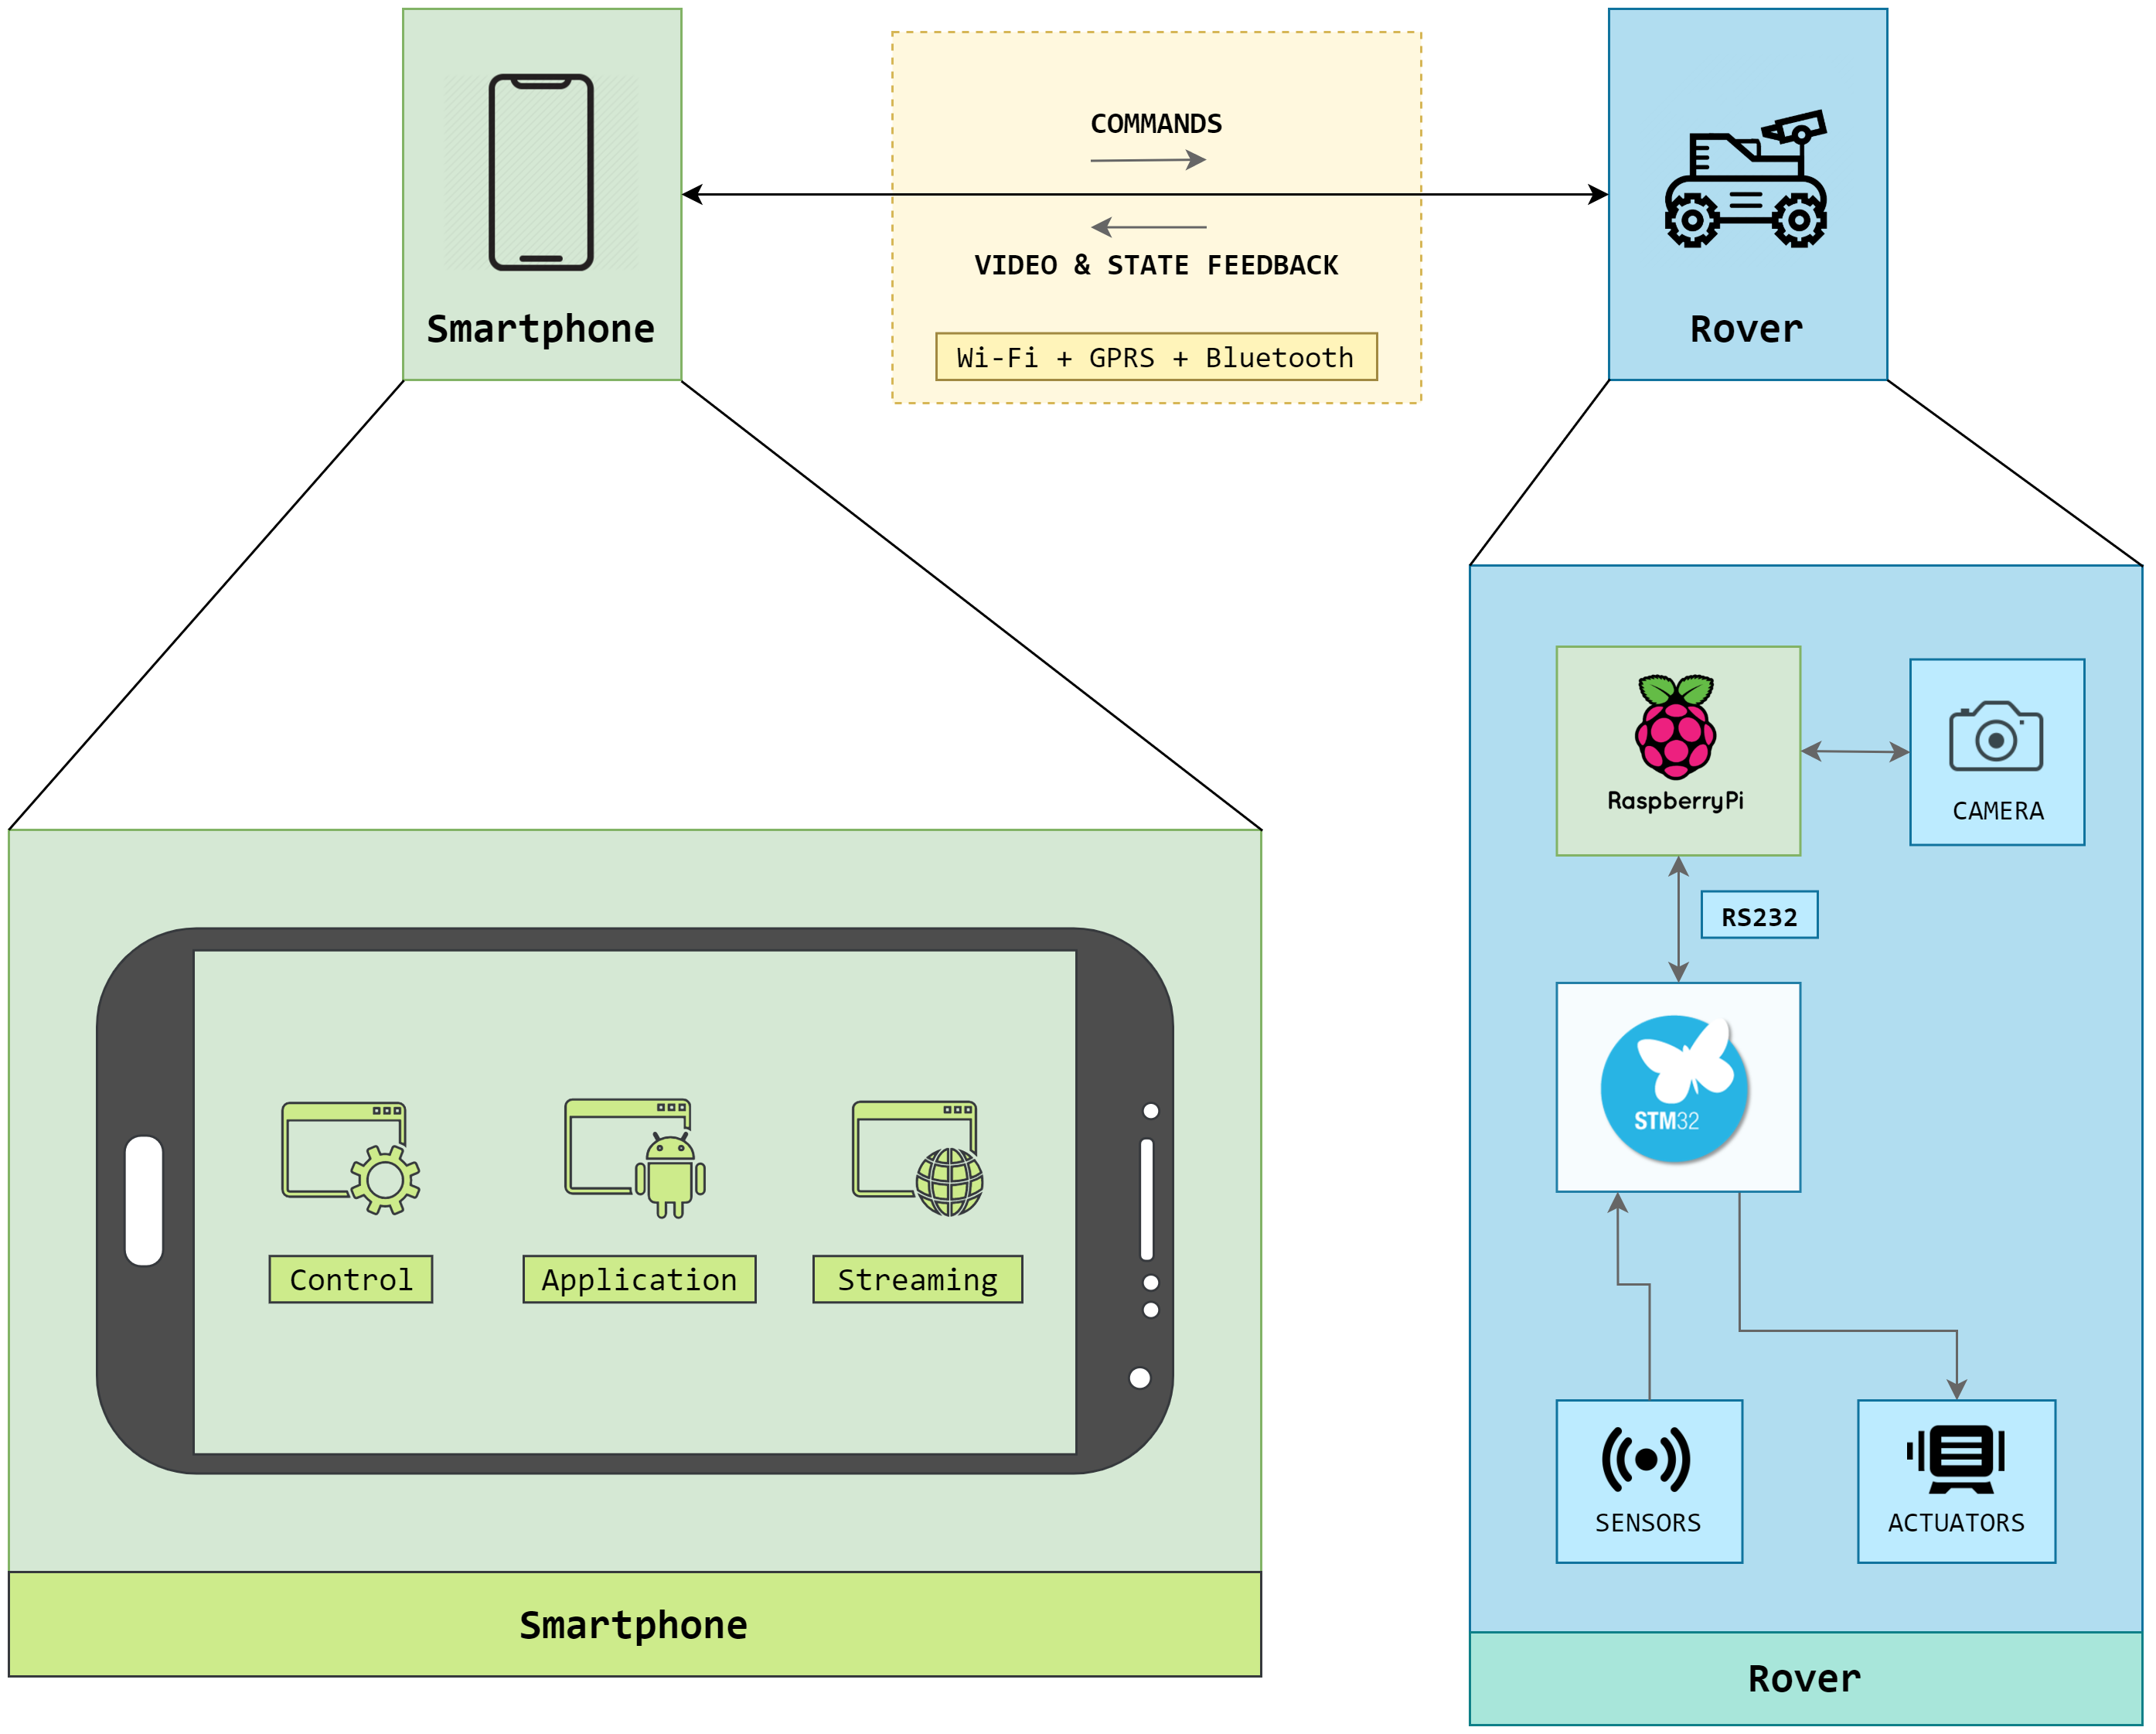
\includegraphics[width=1.0\textwidth]{./img/initial_design_diagram.png}
\caption{\label{fig:initial-design}Initial design: Block diagram view}
\end{figure}
\subsection{Tables}
\label{sec:org333b62a}
\begin{enumerate}
\item Construction: Tables can be created using an online tool
(\url{https://www.tablesgenerator.com/}) and then copied, as illustrated in
\emph{Definition}
\item Definition: 
\lstset{language=[LaTeX]TeX,label= ,caption= ,captionpos=b,numbers=none}
\begin{lstlisting}
% Please add the following required packages to your document preamble:
% \usepackage[table,xcdraw]{xcolor}
\begin{table}[!hbt]
\centering
\caption{Specifications}%
\label{tab:specs-init}
%
\begin{tabular}{
>{\columncolor[HTML]{FFFFFF}}l 
>{\columncolor[HTML]{FFFFFF}}l 
>{\columncolor[HTML]{FFFFFF}}l }
\hline
		& Values     & Explanation                                                                                                  \\ \hline
Autonomy          & 4 h        & \begin{tabular}[c]{@{}l@{}}Time interval between battery fully \\ charged and safely discharged\end{tabular} \\ \hline
Speed Range  & 0.1 to 1 m/s    & \begin{tabular}[c]{@{}l@{}}Speed at which the car can operate\end{tabular}              \\ \hline
Frame Rate        & 60 fps     & \begin{tabular}[c]{@{}l@{}}Frequency at which independent still \\ images appear on the screen\end{tabular}  \\ \hline
Camera Range      & 20 m       & \begin{tabular}[c]{@{}l@{}}How far can the camera capture images\\ without loosing resolution\end{tabular}   \\ \hline
Camera resolution & 480p       & Amount of detail that the camera can capture                                                                 \\ \hline
Communication Range & 50 m & \begin{tabular}[c]{@{}l@{}}Maximum distance between the car and the\\ smarphone without losing connection\end{tabular} \\ \hline
speed Error    & 5 \%       & \begin{tabular}[c]{@{}l@{}}Maximum difference between desired \\ and real speed\end{tabular}              \\ \hline
Direction Error   & 5\%        & \begin{tabular}[c]{@{}l@{}}Maximum difference between desired\\  and real direction\end{tabular}             \\ \hline
Distance Error     & 5 \% & \begin{tabular}[c]{@{}l@{}}Maximum difference between desired\\ and real distance to the obstacle\end{tabular}         \\ \hline
Dimensions        & 20x12x5 cm & Dimensions of the car                                                                                        \\ \hline
Weight            & 0.5 kg     & Weight of the car                                                                                            \\ \hline
\end{tabular}
\end{table}
\end{lstlisting}
\item \textbf{Result}: Table\textasciitilde{}\ref{tab:specs-init} lists the foreseen product
specifications.
\begin{table}[!hbt]
\centering
\caption{Specifications}%
\label{tab:specs-init}
%
\begin{tabular}{
>{\columncolor[HTML]{FFFFFF}}l 
>{\columncolor[HTML]{FFFFFF}}l 
>{\columncolor[HTML]{FFFFFF}}l }
\hline
		& Values     & Explanation                                                                                                  \\ \hline
Autonomy          & 4 h        & \begin{tabular}[c]{@{}l@{}}Time interval between battery fully \\ charged and safely discharged\end{tabular} \\ \hline
Speed Range  & 0.1 to 1 m/s    & \begin{tabular}[c]{@{}l@{}}Speed at which the car can operate\end{tabular}              \\ \hline
Frame Rate        & 60 fps     & \begin{tabular}[c]{@{}l@{}}Frequency at which independent still \\ images appear on the screen\end{tabular}  \\ \hline
Camera Range      & 20 m       & \begin{tabular}[c]{@{}l@{}}How far can the camera capture images\\ without loosing resolution\end{tabular}   \\ \hline
Camera resolution & 480p       & Amount of detail that the camera can capture                                                                 \\ \hline
Communication Range & 50 m & \begin{tabular}[c]{@{}l@{}}Maximum distance between the car and the\\ smarphone without losing connection\end{tabular} \\ \hline
speed Error    & 5 \%       & \begin{tabular}[c]{@{}l@{}}Maximum difference between desired \\ and real speed\end{tabular}              \\ \hline
Direction Error   & 5\%        & \begin{tabular}[c]{@{}l@{}}Maximum difference between desired\\  and real direction\end{tabular}             \\ \hline
Distance Error     & 5 \% & \begin{tabular}[c]{@{}l@{}}Maximum difference between desired\\ and real distance to the obstacle\end{tabular}         \\ \hline
Dimensions        & 20x12x5 cm & Dimensions of the car                                                                                        \\ \hline
Weight            & 0.5 kg     & Weight of the car                                                                                            \\ \hline
\end{tabular}
\end{table}
\#+end\textsubscript{src}
\end{enumerate}

\section{Referencing}
\label{sec:org4dd53de}
To reference the relevant items such as figures, tables, sections (chapter,
section, subsection), etc., one needs:
\begin{enumerate}
\item To label the item, using \texttt{\textbackslash{}label\{<item>:<item-name>\}}:
e.g. \texttt{\textbackslash{}label\{ch:analysis\}}
\item Then, one can reference it using: \texttt{\textbackslash{}ref\{<item>:<item-name>\}}:
e.g. Chapter\textasciitilde{}\ref{ch:analysis}
\end{enumerate}
\section{Bibliography}
\label{sec:org6b2f0b5}
Bibliography management is composed of 2 parts:
\begin{enumerate}
\item A Bibliography database, generally a \texttt{.bib} file, located at
\texttt{./bib/dissert.bib} (see \href{file:///Users/zemiguel/Documents/Univ/MI\_Electro/Sem6/LPI2/PI/github/Deliverables/Final/bib/dissert.bib}{here})
\begin{itemize}
\item Example of Bibliography entry
\lstset{language=[LaTeX]TeX,label= ,caption= ,captionpos=b,numbers=none}
\begin{lstlisting}
@article{harashima1996mechatronics,
  title={Mechatronics-" What Is It, Why, and How?" An Editorial},
  author={Harashima, Fumio and Tomizuka, Masayoshi and Fukuda, Toshio},
  journal={IEEE/ASME Transactions on Mechatronics},
  volume={1},
  number={1},
  pages={1--4},
  year={1996},
  publisher={IEEE}
}
\end{lstlisting}
\item Bibliography entry can be created as:
\begin{itemize}
\item Search the topic at \url{https://scholar.google.pt/}.
\item Select the Export To Bibtex option
\item Copy to the \texttt{.bib} file
\end{itemize}
\end{itemize}
\item A citation, using \texttt{\textbackslash{}cite\{<bib-key>\}}, where \texttt{<bib-key>} is the key defined in
the \texttt{.bib} file. 
\begin{itemize}
\item For example: Mechatronics, was defined by Harashima
et. al=\textasciitilde{}\cite{harashima1996mechatronics}=
\end{itemize}
\end{enumerate}
\section{Enviroments}
\label{sec:orgd96ea1a}
\subsection{Itemize}
\label{sec:orga57400f}
\lstset{language=[LaTeX]TeX,label= ,caption= ,captionpos=b,numbers=none}
\begin{lstlisting}
\begin{itemize}
\item \textbf{Item 1}: this is an item
\item \textbf{Item 2}: this is another item
\end{itemize}
\end{lstlisting}
\textbf{Result}:
\begin{itemize}
\item \textbf{Item 1}: this is an item
\item \textbf{Item 2}: this is another item
\end{itemize}

\subsection{Enumerate}
\label{sec:org56418de}
\lstset{language=[LaTeX]TeX,label= ,caption= ,captionpos=b,numbers=none}
\begin{lstlisting}
\begin{enumerate}
\item \textbf{Item 1}: this is an enumerated item
\item \textbf{Item 2}: this is another enumerated item
\end{enumerate}
\end{lstlisting}
\textbf{Result}:
\begin{enumerate}
\item \textbf{Item 1}: this is an enumerated item
\item \textbf{Item 2}: this is another enumerated item
\end{enumerate}

\section{Glossary}
\label{sec:org4fa9b69}
Glossaries are useful to input \uline{acronyms} and \uline{symbols}.
\begin{itemize}
\item Acronyms: common use words, often abbreviated.
\item Symbols: mathematical/physical symbols that usually require some brief
description and the relevant units.
\end{itemize}

Glossary management is composed of 3 parts:
\begin{enumerate}
\item A Glossary database 
\begin{itemize}
\item Acronyms: \texttt{./sec/acronyms.tex}
\item Symbols: \texttt{./sec/symbols.tex}
\end{itemize}
\item A reference using \texttt{\textbackslash{}gls\{<gls-key>\}}, where \texttt{<gls-key>} is the key defined in
the glossary database file.
\item An external utility that manages the glossary entry items addition and
referencing (no need to worry about this, the makefile will handle it).
\end{enumerate}
\subsection{Acronyms}
\label{sec:org00ca075}
\begin{itemize}
\item Definition (\texttt{./sec/acronyms.tex}):
\lstset{language=[LaTeX]TeX,label= ,caption= ,captionpos=b,numbers=none}
\begin{lstlisting}
\newacronym{sls}{SLS}{Selective Laser Sintering}
\newacronym{slm}{SLM}{Selective Laser Melting}
\end{lstlisting}
\item Usage: These are two acronyms used together: \texttt{\textbackslash{}gls\{sls\}/\textbackslash{}gls\{slm\}} technology.
\end{itemize}

\subsection{Symbols}
\label{sec:org33b2693}
\begin{itemize}
\item Definition (\texttt{./sec/symbols.tex}):
\lstset{language=[LaTeX]TeX,label= ,caption= ,captionpos=b,numbers=none}
\begin{lstlisting}
\newglossaryentry{omega}
{
    name={\ensuremath{\omega}},
    description={angular velocity},
    sort=omega,
    symbol={\ensuremath{\omega}},
    unit={\si{rad/s}}
}
\end{lstlisting}
\item Usage: this is \texttt{\textbackslash{}gls\{omega\}}.
\end{itemize}

\section{Listings}
\label{sec:orga636528}
\begin{itemize}
\item Styling: Listings can be formatted using different styles, as presented in
\texttt{./sty/listing.sty} for any programming/markup language required.
\begin{itemize}
\item Example: C
\lstset{language=[LaTeX]TeX,label= ,caption= ,captionpos=b,numbers=none}
\begin{lstlisting}
\lstdefinestyle{customc}{
belowcaptionskip=1\baselineskip,
breaklines=true,
%frame=L,%lines, whole
xleftmargin=\parindent,
language=C,
showstringspaces=false,
basicstyle=\scriptsize\ttfamily,
keywordstyle=\bfseries\color{green!40!black},
commentstyle=\itshape\color{purple!40!black},
identifierstyle=\color{blue},
stringstyle=\color{orange},
numberstyle={\tiny},
numbers=left,
numberblanklines=false,
stepnumber=5,
backgroundcolor=\color{yellow!10}, 
frame=tlb
}
\end{lstlisting}
\end{itemize}
\item Usage: Listings can be inputted using the desired style as below. It includes
a caption, a label, a style, and a file path:
\lstset{language=[LaTeX]TeX,label= ,caption= ,captionpos=b,numbers=none}
\begin{lstlisting}
\lstinputlisting[language=C++, caption={Thread Serial Rx handler},label=lst:threadSerialRx,
style=customc]{./listing/threadSerialRx.cpp}%
\end{lstlisting}
\item Result:
\end{itemize}
\lstset{language=C,label= ,caption= ,captionpos=b,numbers=none,style=customc}
\begin{lstlisting}
UINT MMSLSDlg::ThreadSerialRx(LPVOID param)
{
    /* Wait for 1st connection to serial port: OnConnect */
    ::WaitForSingleObject( EvSerial.m_hObject , INFINITE); 
    tstring szData;
    CDemoEzdDlg *dlg = (CDemoEzdDlg *)param;

    while(1)
    ;

    return 0;
}
\end{lstlisting}
\section{PDF inclusion}
\label{sec:org738167b}
\begin{itemize}
\item Include all pages from \texttt{anexo3-license}. Be careful of file path. It's
relative to the main file.
\lstset{language=[LaTeX]TeX,label= ,caption= ,captionpos=b,numbers=none}
\begin{lstlisting}

\includepdf[pages=-]{anexo3-license}
\end{lstlisting}
\end{itemize}
\section{Appendices}
\label{sec:org04315bb}
Appendices can be added in the appropriate section (\texttt{./tex/Append/}):
\begin{itemize}
\item as text: with figures, tables, etc.
\item included as PDF
\end{itemize}
\end{document}